\begin{frame}
\frametitle{Decoherence}
\begin{columns}
  \begin{column}{0.5\textwidth}
    \textbf{Energy loss into materials}
    \begin{align*}
      \text{start: }& \ket{1}\ket{0} \equiv \ket{10} \\
      \text{interact: }& \cos(g t) \ket{10} + \sin(g t) \ket{01}\\
      \text{reduce: }& P_{\ket{1}} = \cos(g t)^2, \, P_{\ket{0}} = \sin(g t)^2
    \end{align*}
    Bath of defects, exponential decay: $P_{\ket{1}} = \exp(-t/T_1)$
  \end{column}
  \begin{column}{0.5\textwidth}
    \begin{figure}
      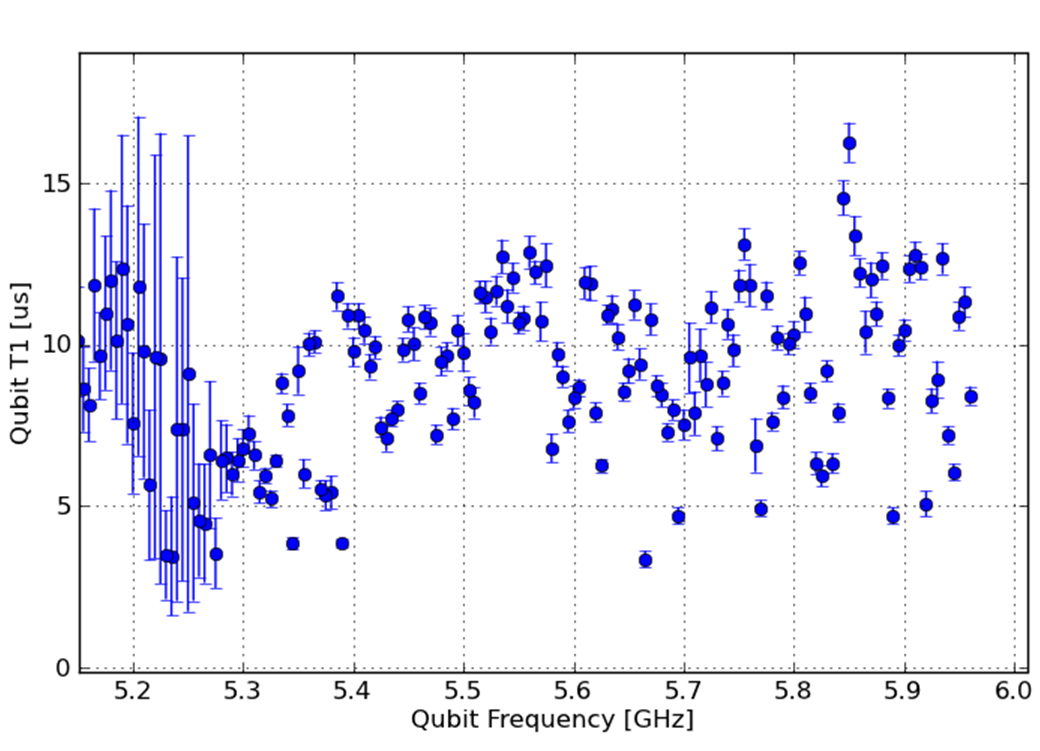
\includegraphics[scale=0.3]{t1_versus_frequency.png}
      \caption*{Frequency spectrum of material defects}
    \end{figure}
  \end{column}
\end{columns}
\pause
\begin{columns}
  \begin{column}{0.2\textwidth}
    \textbf{Dephasing}
    \begin{figure}
      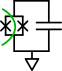
\includegraphics{transmon_magnetic_noise.pdf}
    \end{figure}
  \end{column}
  \begin{column}{0.8\textwidth}
    \begin{itemize}
        \item $\ket{0} + \underbrace{\exp \left( i \int \omega(t) \, dt \right)}_\text{uncertain} \ket{1}$
        \item Classical uncertainty in quantum phase.
        \item Comes from spin moments on metal surface.
    \end{itemize}
  \end{column}
\end{columns}
\end{frame}
